\chapter{Airplanes}

Now that you understand how a sail works,  you are ready to understand how an airplane works.   

\section{Drag and Thrust}

As airplane flies,  the air around it creates a big force that is trying to slow the 
plane down.  Pilots call this \newterm{drag}.


To overcome drag,  an airplane must have a source of \newterm{thrust}.  This is usually done by pushing air toward the back of plane.

There are basically three types of propulsion on airplanes:

\begin{itemize}
\item Propeller planes have fan blades that are spun by an internal combustion engine and push the air toward the back of the plane.  
\item Jet planes suck air into a tube,  mix it with fuel,  and ignite the mixture.  There are fan blades inside the tube that ensure
the power from the burn is efficiently converted into thrust.
\item Turboprop planes use both propeller and jet technology: they have propellers turned by jet engines.
\end{itemize}

Drag is proportional to the square of the velocity.  So, for example,  if you fly twice as fast,  the drag force will increase by a factor of 4. 

Passenger airplane fly fast -- they have no trouble reaching 1000 km per hour.   A Boeing 747 burns about 4 liters of fuel per second; the flight from London to New York requires about 70,000 kg of fuel.  When the plane takes off,  the fuel for the journey often weighs twice as much as the passengers.
 
\section{Lift}

Unlike a hot air balloon,   an airplane is heavier than the 
air it displaces,   so the force of gravity will pull it from the sky unless there is a counteracting force.  We call the counteracting force \newterm{lift}.

Lift works just like a sailing into the wind: By picking an angle of attack,   we create high pressure under the wing.  By creating a nice smooth path for the 
air to travel over the top of the wing,  we create low pressure over the wing.  This difference creates the lift on the wings.

PICTURE HERE:

(There are some very bad explanations of this idea that overstate the importance of the rounded top of the wing.   Most airplanes can fly upside down -- if the 
most important part were the shape of the top,  this would be impossible.  The most important part is the angle of attack.)

At high altitudes,  the air is less dense.  If two identical planes are flying  at the same speed,  but at different altitudes,: 
\begin{itemize}
\item There is less drag on the higher airplane.
\item The wings provide less left on the higher airplane.
\item The air around the higher plane has less oxygen per liter,  which can affect how the fuel burns.
\end{itemize}

\section{Control}

The first control that a pilot has is the throttle.   By increasing the throttle,  the pilot increases the plane's thrust.

The pilot has a stick.  Pulling back on the stick causes the \newterm{elevator} on the tail of the plane to go up.  Air hitting the elevator pushes the tail down and the nose up. 


Pushing the stick forward will push the tail up and the nose down.  We say "The elevator controls the \newterm{pitch} of the airplane."

The stick also goes left and right.   Pushing the stick to the left,  lifts the \newterm{aileron} on the left wing and lowers the aileron on the right wing.  This pushes the left wing down and 
pushes the right wing up.  We say "The ailerons control the  \newterm{roll} of the airplane."

The pilot controls the \newterm{rudder} on the tail with his feet.   Pushing the right side down will push the rudder to the right.  This will push the tail of the plane to the left and the 
nose to the right.  We say "The rudder controls the \newterm{yaw} of the airplane."


\section{Thrust}

There are several common ways that airplanes produce thrust.

The first is a propeller powered by a standard piston engine.

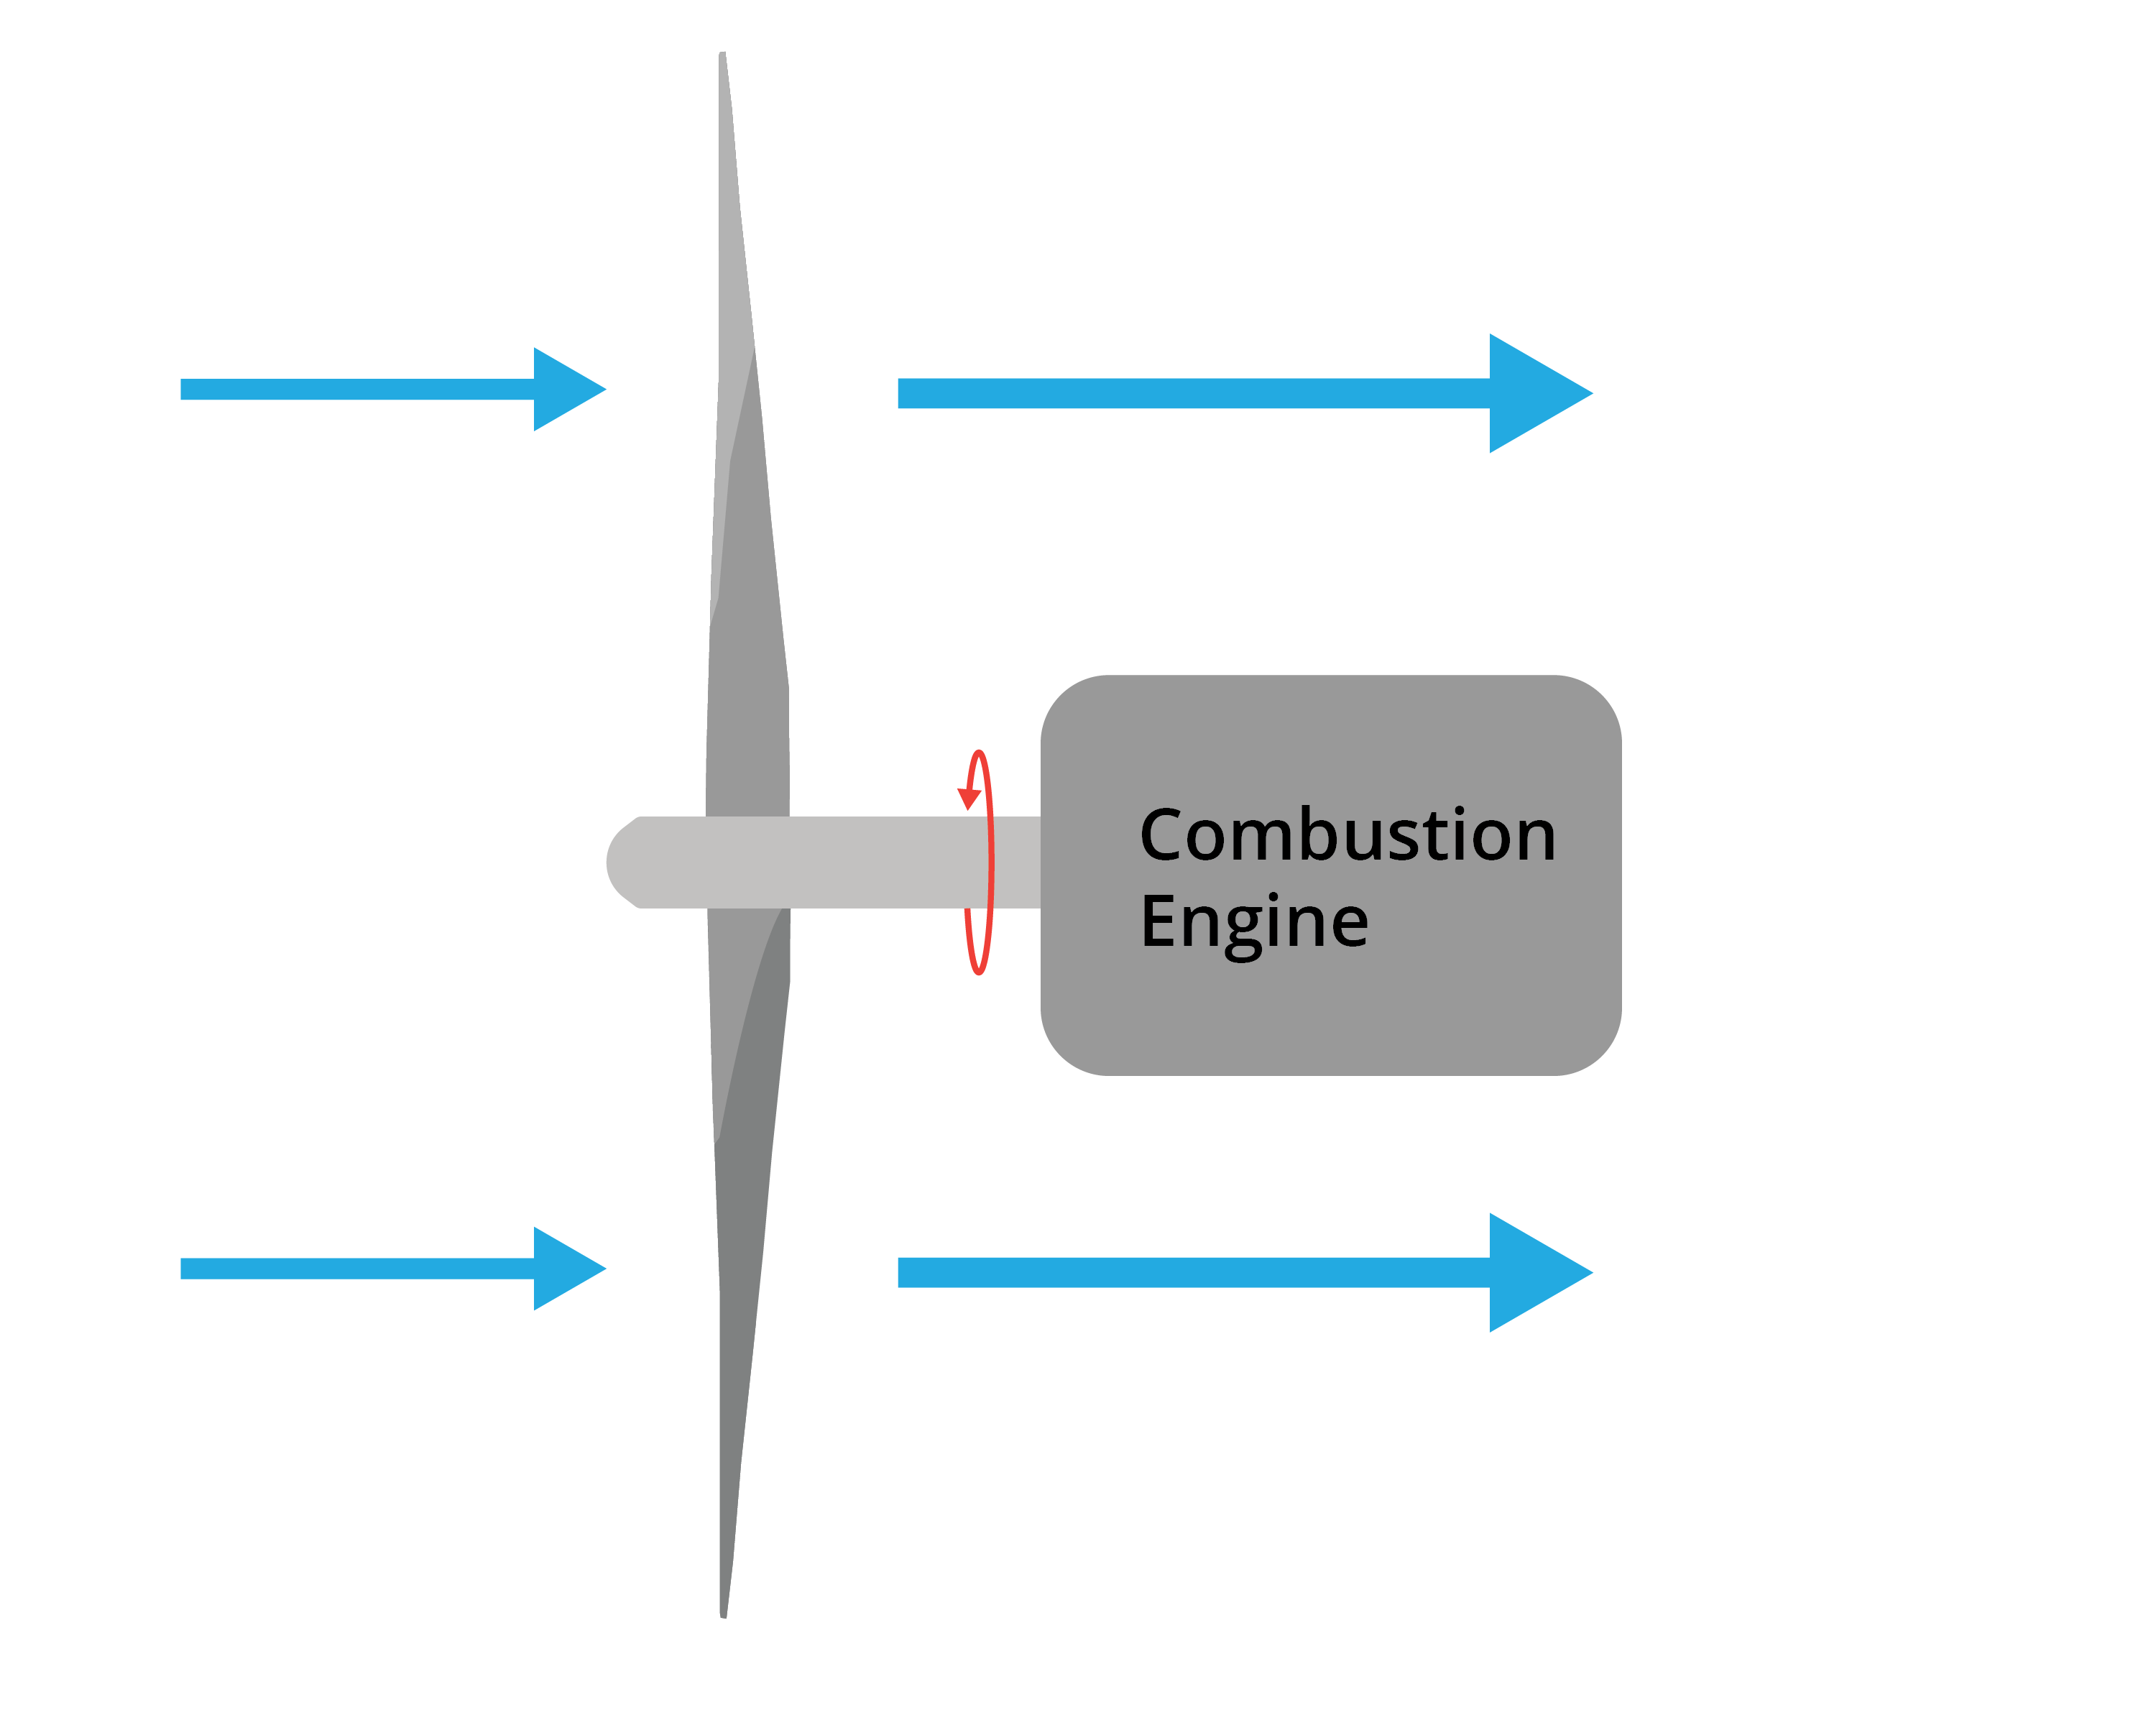
\includegraphics[width=0.75\textwidth]{propeller.png}

The propeller [HOW PROPELLER USES PRESSURE]


Another way to produce thrust is by using a \newterm{jet engine}. Jet engines take in air, and increase its pressure and temperature, and shoots it out of the back of the engine. The combination of making air move much faster while also 

and XXX can make a jet engine more powerful than standard pistol-driven propellers. 


Jet engines suck in air, compress it, add a fuel mixture, ignite the fuel, and shoot it out the back. Once the air exits the engine, it expands at a high speed, which further helps create thrust. 




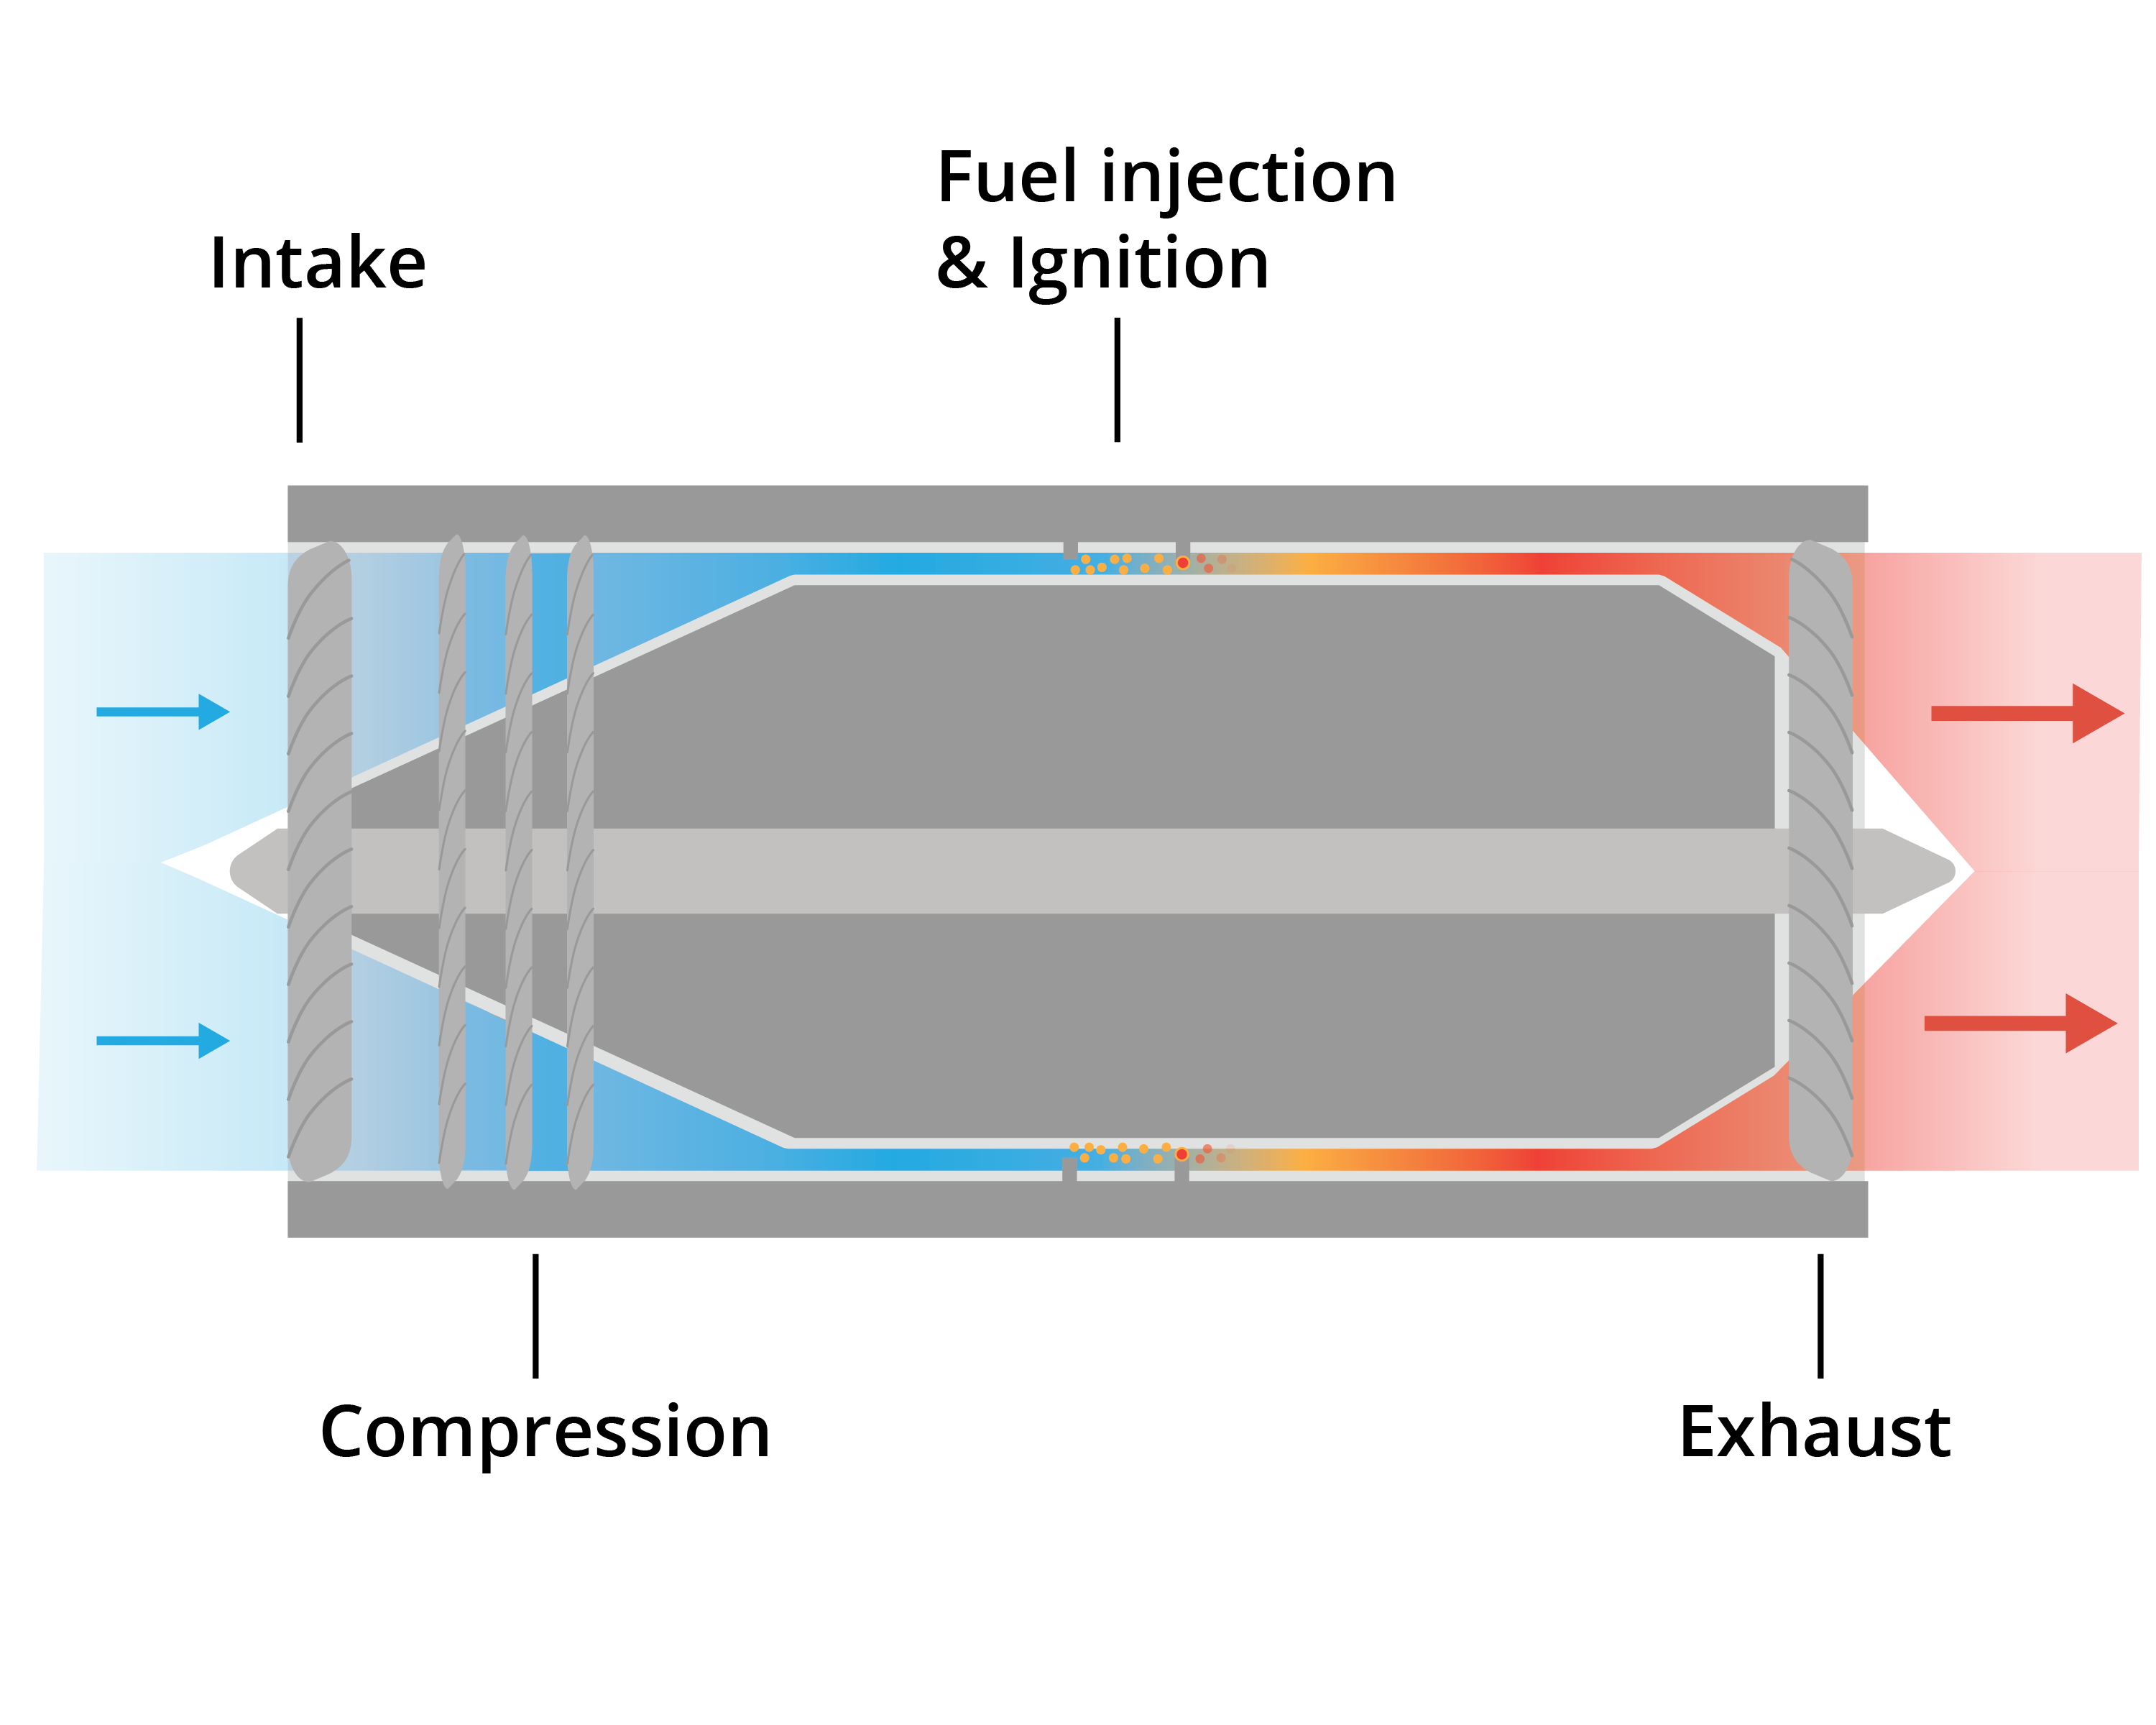
\includegraphics[width=0.75\textwidth]{jet.png}



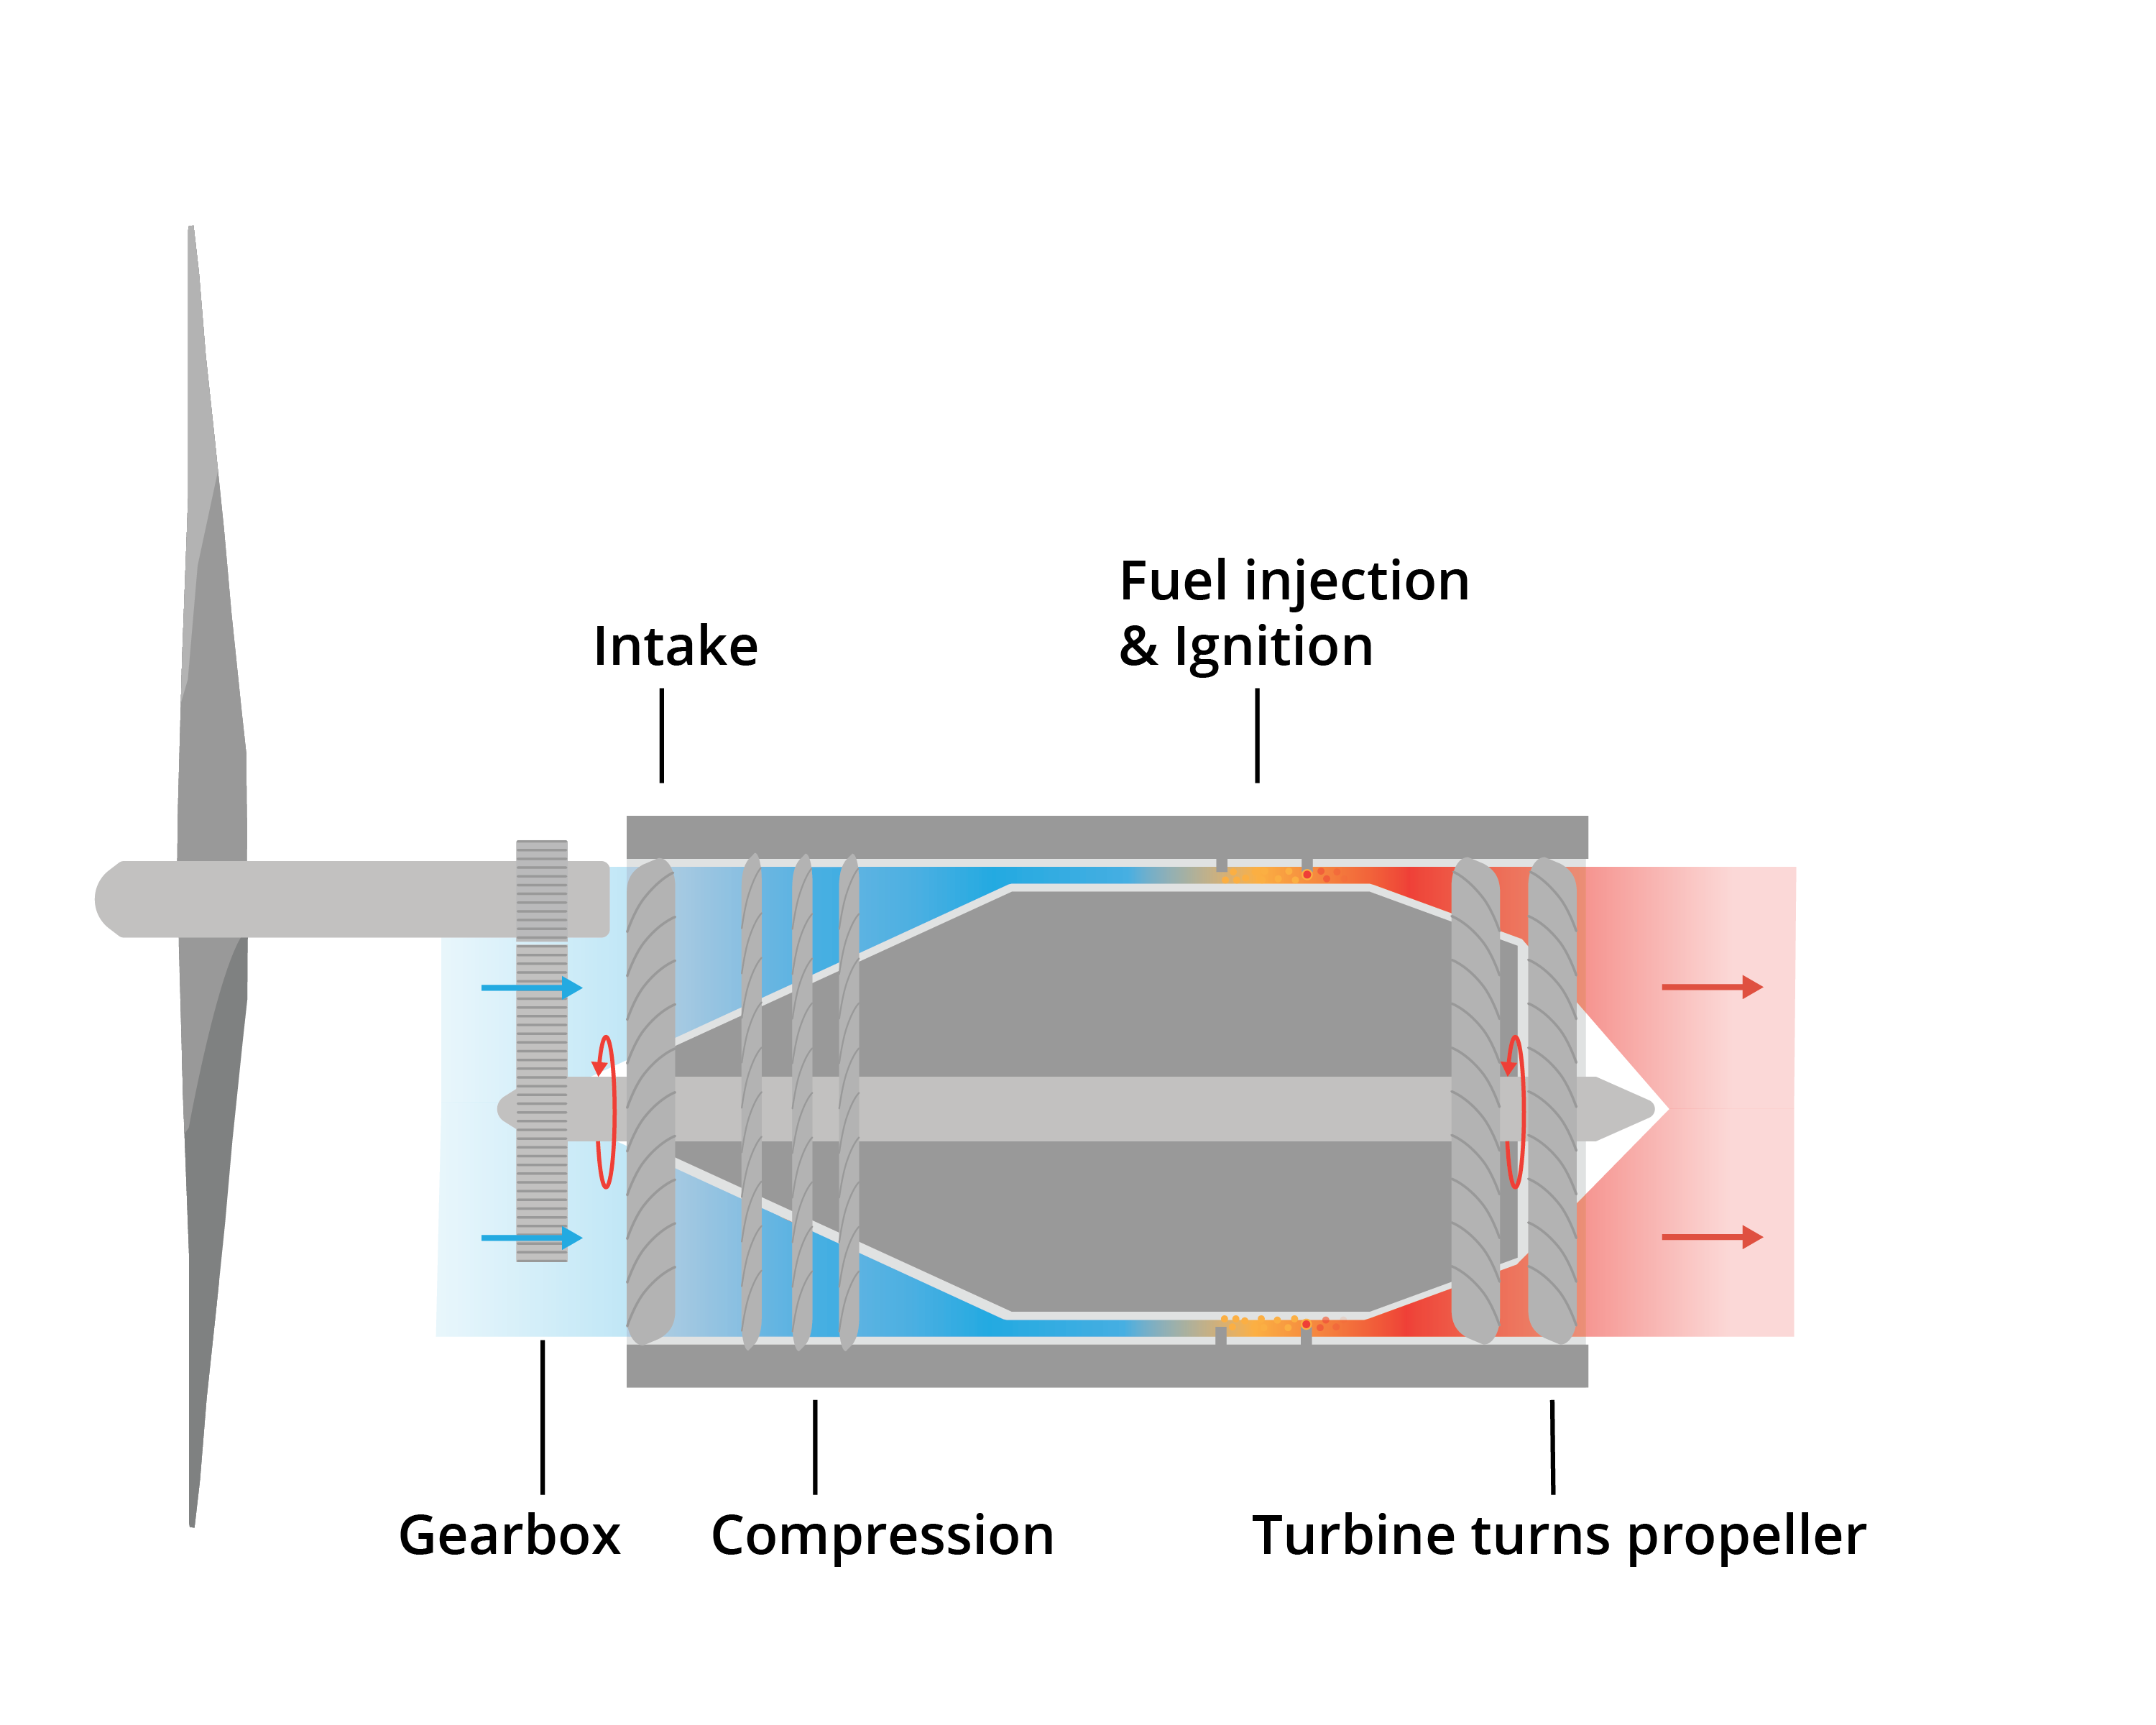
\includegraphics[width=0.75\textwidth]{turboProp.png}


\section{Gliders}

It is interesting to note that gliders fly with no engines.   Gliding usually starts high in the air,  where the glider has lots of potential energy.   To stay aloft for a long
time,  glider pilots will look for places where air is rising -- so they can ride those updrafts and regain that potential energy.

